
\chapter{La idea del reloj, un poco más precisa}

\lettrine[ante=\raisebox{-1.5ex}{\Large ---},lines=2]{B}{ien, Cecilia}
---comenzó Antonia, con gesto a\-dus\-\mbox{to---;} ahora sí la cosas empezarán a
complicarse.

---¡Por fin! ---exclamó Cecilia, simulando una confianza en sí misma
que no estaba tan segura de sentir.

---Antes de sumergirnos definitivamente en nuestro reloj, aún debemos
conquistar unas pocas herramientas más de \openscad{}; pero creo que
éste es un buen momento para justificarlas previamente precisando un
poco más nuestro objetivo ---Antonia desgranaba su explicación con
lentitud; Cecilia temió que estuviera por caer en una de sus tantas
procrastinaciones: cuando estaba a punto de terminar un proyecto,
empezaba a dar vueltas y más vueltas, como si concluir algo (cualquier
cosa que fuere) supusiera una pérdida o una despedida que quisiera
evitar o demorar---. El cuerpo principal de nuestro reloj, como
dijimos, será un semicilindro:

%  \begin{center}
    \begin{lstlisting}
module cuerpo(largo,
              radio,
              center=false){
  rotate([-90,0,0])
    semicilindro(h=largo,
                 r=radio,
                 center=center,
                 $fn=200);
}
cuerpo(150,30,center=true);
    \end{lstlisting}%$
%  \end{center}

  \begin{figure}[ht]
    \centering
    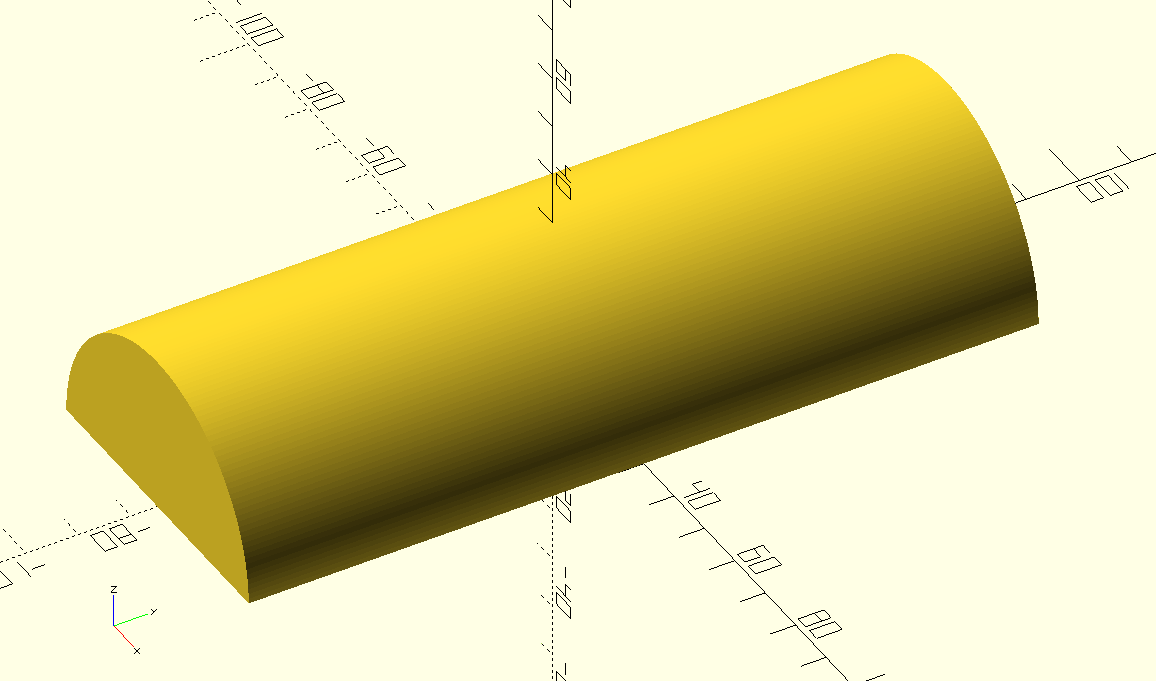
\includegraphics[width=.7\textwidth]{imagenes/cuerpo-base-reloj}
      \caption{El cuerpo del reloj.}
      \label{fig:cuerpo-base-reloj}
    \end{figure}

      
    \guillemotright Luego revisaremos las medidas ---aclaró---; usé
    esos valores sólo para fijar ideas.

    ---¡Pasaste el
    \lstinline!$fn=200! como parámetro del semicilindro en la línea 8!
    ---Cecilia estaba muy atenta.%$

    ---Ah, sí; no te conté ---reconoció Antonia---; es una posibilidad
    muy interesante: si hacés eso, la variable \lstinline!$fn! sólo
    aplica al cuerpo que la recibe. De esa forma, no obligás a todos
    tus objetos a respetar la misma configuración.

    \guillemotright Ahora bien ---Antonia avanzó a tientas, como quien
    busca la mejor forma de una idea---; supongamos que podemos
    determinar la dirección del Sol en un momento dado del día... y lo
    seremos, por supuesto: ¡al final, somos astrónomas! ---sonrió, y
    Cecilia le devolvió la sonrisa, alentándola a continuar---.
    Entonces, deberemos cortar el cuerpo principal con unos
    paralelepípedos orientados según esa dirección, como los de las
    figuras \ref{fig:digitos-cortes}.

  \begin{figure}[t]
    \centering
    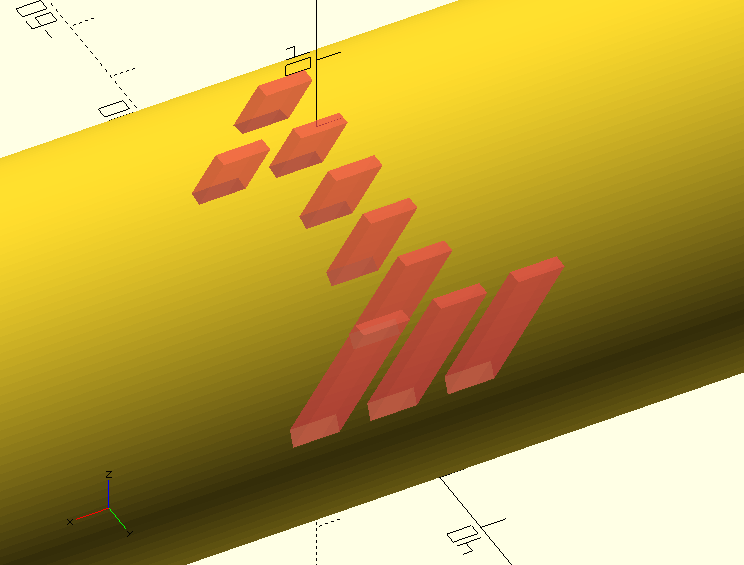
\includegraphics[width=.49\textwidth]{imagenes/digito-corte-1}\hfill
    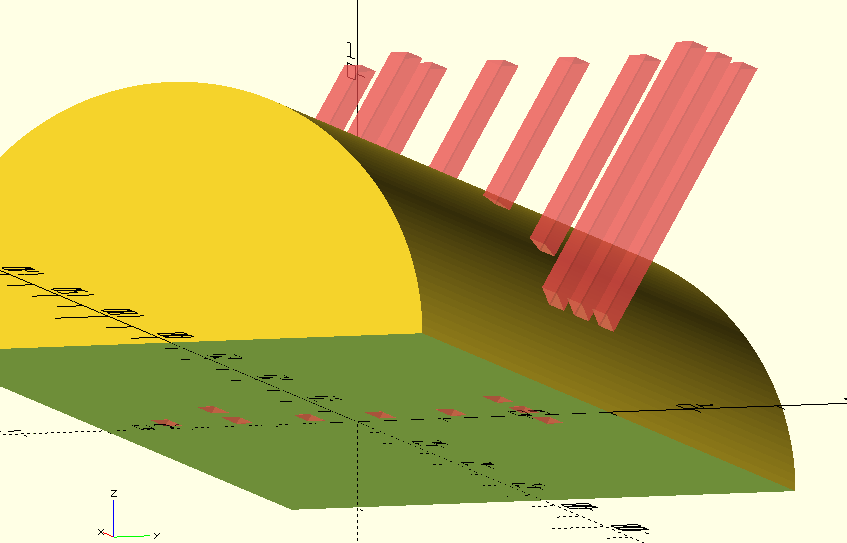
\includegraphics[width=.49\textwidth]{imagenes/digito-corte-2}
        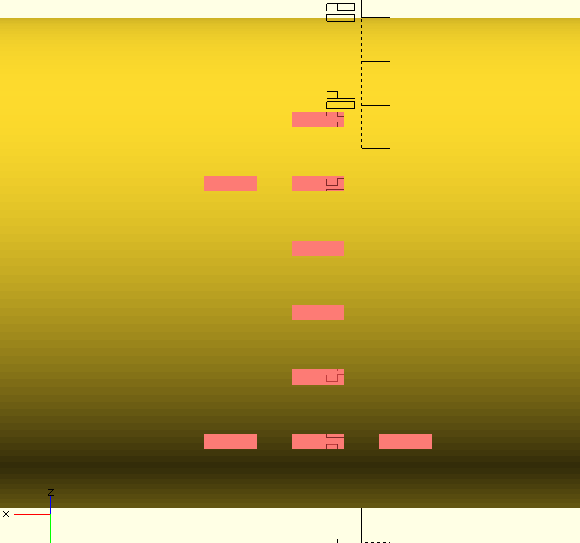
\includegraphics[width=.5\textwidth]{imagenes/digito-corte-3}
        \caption{Palalelepípedos con los que Antonia propone horadar
          el cuerpo del reloj, a fin de formar los dígitos que
          señalarán la hora. Podemos considerar al Sol tan lejos de
          la Tierra que sus rayos llegarán al reloj de manera paralela
          entre sí.}
    \label{fig:digitos-cortes}
  \end{figure}

  Los ojos de Cecilia parecían querer comerse el monitor. Lo que allí
  pasaba era demasiado hermoso para ser verdad... y también demasiado
  arduo. De pronto, en un vértigo, sintió que no podría repetir, ni
  aún siquiera comprender, lo que allí estaba
  ocurriendo. Instintivamente giró sobre sí misma para mirar a
  Antonia: esperaba encontrar en ella la seguridad que le faltaba,
  pero sorprendió en sus ojos un reflejo de su propia e incipiente
  angustia. Comprendió ---conociéndola como la conocía--- que ella
  también estaba preocupaba: el fantasma de ser una impostora como
  docente siempre la acechaba. Así que ahí estaban las dos: angustiada
  una por poder entender, y la otra por saber explicar. Cecilia supo
  entonces que la única salida que tenían debía recorrerse juntas:
  aliadas frente al mismo problema.

  Antonia no pudo seguir, naturalmente, el pensamiento de su amiga,
  pero algo debió intuir cuando finalmente la vio sonreír, porque
  inmediatamente su rostro se despejó y los rayos de una tímida
  sonrisa destellaron en él.

    \begin{figure}[t]
    \centering
    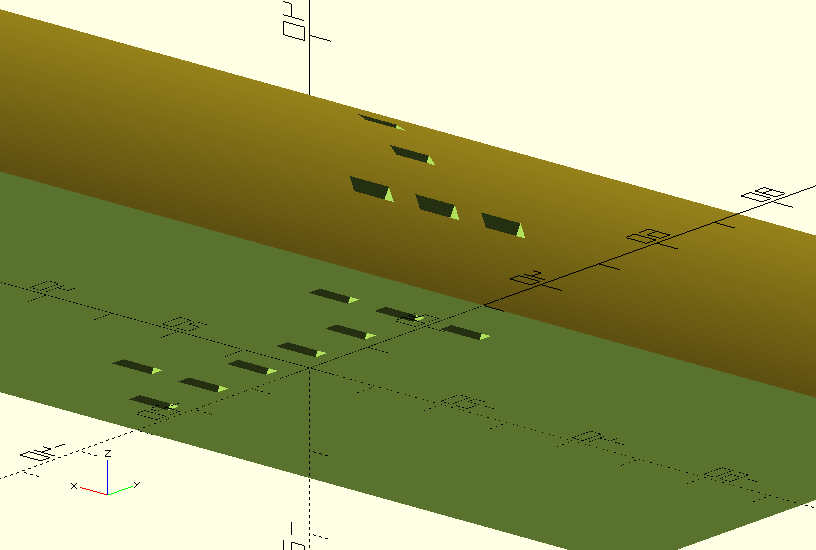
\includegraphics[width=.7\textwidth]{imagenes/digito-corte-4}
    \caption{Agujeros que forman el dígito \texttt{1}.}
    \label{fig:digito-corte-limpio}
  \end{figure}

  ---Si borro efectivamente los paralelepípedos quedaría como en la
  figura \ref{fig:digito-corte-limpio} ---dijo.


  ---Hermoso ---pronunció esta vez Cecilia en voz alta, con la
  seguridad de que juntas podrían hacer no sólo un reloj, sino un
  almanaque entero si hacía falta.



%%% Local Variables:
%%% mode: latex
%%% TeX-master: "../libro"
%%% End:
